\chapter{Introducción específica} % Main chapter title

\label{Chapter2}

%----------------------------------------------------------------------------------------
%	SECTION 1
%----------------------------------------------------------------------------------------
En este capítulo se hace mención a las partes constituyentes del dispositivo de adquisición de señales neurofisiológicas, se introduce a su hardware y al stack Bluetooth. Adicionalmente se muestran las herramientas de desarrollo utilizadas en el proyecto.

\section{Hardware del DASN}
\label{sec:Hard}
El DASN está integrado en una sola placa y es un dispositivo portátil alimentado por baterías. Su arquitectura está basada en dos circuitos integrados principales, el microcontrolador CC2640R2 y \textit{Analog front end} (AFE) ADS1299. Los AFE son dispositivos que incorporan la parte analógica para el acondicionamiento de la señal y el conversor analógico digital para poder digitalizar la señal. En la figura \ref{fig:diagBloquesHardware} se puede ver un diagrama en bloques del hardware.

\vspace{1cm}

\begin{figure}[htbp]
	\centering
	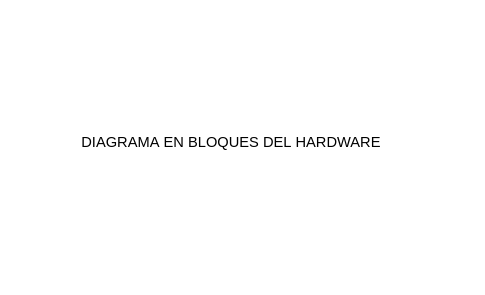
\includegraphics[width=1\textwidth]{./Figures/DiagramaEnBloquesHardware.png}
	\caption{Diagrama en bloques del hardware.}
	\label{fig:diagBloquesHardware}
\end{figure}

\vspace{1cm}

\subsection{Circuito de entrada}
el circuito de entrada del DASN está basado en un circuito integrado ADS1299 \citep{PART:ADS1299}, como se explicó en la sección \ref{sec:Hard} es un AFE. En particular el ADS1299 es un dispositivo de 8 canales, 24 bits por canal, conversión analógica digital sigma delta simultánea, con amplificadores de ganancia programable y un circuito multiplexor que permite conectar las entradas de múltiples formas que lo hacen ideal para el registro de biopotenciales y en particular de señales de EEG. En la figura \ref{fig:diagBloquesADS1299} se puede ver el diagrama en bloques del ADS1299

\vspace{1cm}

\begin{figure}[htbp]
	\centering
	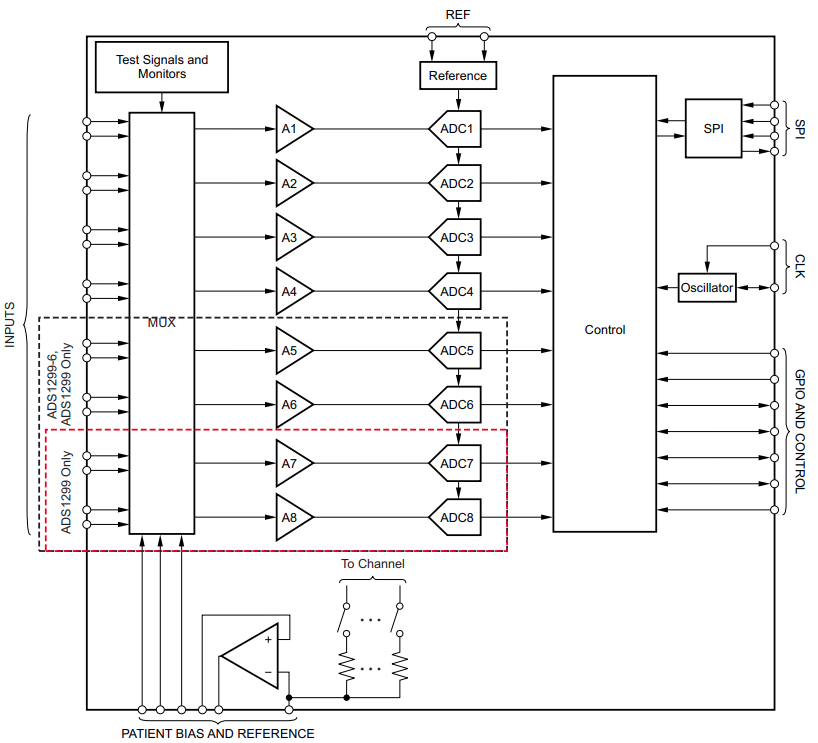
\includegraphics[width=1\textwidth]{./Figures/DiagramaEnBloquesADS1299.png}
	\caption{Diagrama en bloques del ADS1299 \protect\footnotemark.}
	\label{fig:diagBloquesADS1299}
\end{figure}

\vspace{1cm}
\footnotetext{Imagen tomada de la hoja de datos del ADS1299 \citep{PART:ADS1299}.}

El ADS1299 posee un puerto de comunicación SPI. Adicionalmente se dispone de señales de control para poder configurar y controlar el dispositivo. El microcontrolador del DASN está conectado a todas estas interfaces de control del ADS1299.

El DASN posee un canal de potenciales evocados. Esta señal tiene una amplitud menor al ruido de entrada del ADS1299. Para poder medir este biopotencial el DASN incorpora un amplificador entre el paciente y el AFE para adaptar los niveles de la señal. El resto de los canales solo incorporan un filtro de radiofrecuencia pasivo. 

Debido al amplificador extra que incorpora el canal de potenciales evocados, no se puede medir la impedancia de los electrodos de este canal con la señal de impedancia que genera el AFE ya que no se está en contacto con el paciente.

\subsection{Microcontrolador y comunicación inalámbrica}
El DASN posee un microcontrolador CC2640R2 con arquitectura Arm® Cortex®-M3. Este microcontrolador posee integrado un \textit{tranceiver} de 2.4 GHz compatible con la tecnología Bluetooth de baja energía 5.1 y versiones anteriores del stack Bluetooth \citep{PAPER:STACKBLE}. El hecho de tener este tipo de microcontrolador con el \textit{tranceiver} integrado permite configurar el stack Bluetooth por completo, con lo que se logran mejores prestaciones en consumo y ancho de banda al poder elegir el protocolo de comunicación y el modo de trabajo. La placa del DASN posee una antena tipo F \citep{PAPER:ANTENAF} integrada en el circuito impreso y también ofrece la posibilidad de conectar una antena externa. 

\subsection{Conceptos básicos del stack Bluetooth 5.0}
\label{subsec:ConceptosBLE}
%Saco el siguiente párrafo por recomendación de Matias.
%Se darán algunos conceptos básicos sobre el stack Bluetooth ya que ayudarán a entender las configuraciones realizadas que se verán en el siguiente capítulo. A lo largo de la memoria se usan los nombres en inglés ya que muchos términos no tienen traducción y la mayoría de la bibliografía así los referencia. 
El Bluetooth de baja energía, también conocido por sus siglas en inglés como BLE, se divide en distintas capas. La aplicación de usuario entra en contacto con las dos capas superiores del stack Bluetooth, la capa GAP y la capa GATT. A través de estas capas es que el software del DASN configura y maneja la comunicación BLE.

\subsubsection{Capa GAP}
La capa GAP del stack Bluetooth es responsable de las conexiones. De acuerdo a la definición de esta capa un dispositivo Bluetooth se puede encontrar en uno de los siguientes estados:

\begin{itemize}
\item \textit{Standby}: el dispositivo se encuentra en el estado inactivo inicial al reiniciarse.
\item \textit{Advertising}: el dispositivo se anuncia con datos específicos que le permiten a cualquier dispositivo saber que es un dispositivo conectable. Este anuncio contiene la dirección del dispositivo y puede contener algunos datos adicionales, como el nombre del dispositivo.
\item \textit{Scanning}: se escuchan los mensajes enviados por algún \textit{advertiser}.
\item \textit{Initiating}: se inicia la conexión, pero el \textit{advertiser} es quien dependiendo los datos enviados por el \textit{initiator} acepta o no la conexión.
\item \textit{Connected}: Cuando se establece una conexión entre ambos dispositivos.
\end{itemize}

A su vez, la capa GAP define cuatro roles para los dispositivos [ref]:

\begin{itemize}
\item \textit{Broadcaster}: es un anunciante que no se puede conectar.
\item \textit{Observer}: busca anuncios pero no puede iniciar conexiones.
\item \textit{Peripheral}: es un anunciante que se puede conectar y funciona como \textit{peripheral} en una conexión de una sola capa de enlace.
\item \textit{Central}: busca anuncios e inicia conexiones y funciona como central en una o varias conexiones.
\end{itemize}

\subsubsection{Capa GATT}
La capa GATT es usada por la aplicación para el envío y recepción de los datos. Los datos son pasados y almacenados desde la aplicación de usuario al \textit{stack} Bluetooth en forma de características. La capa GATT define los siguientes roles para los dispositivos que se encuentran conectados:
\begin{itemize}
\item GATT \textit{server}: Es el dispositivo que tiene el espacio de memoria para la información que va a ser leída o escrita por un GATT \textit{client}.
\item GATT \textit{client}: Es el dispositivo que lee o escribe información de un GATT \textit{server}.
\end{itemize}

Los roles de la capa GATT (\textit{client} o \textit{server}) son independientes de los roles de la capa GAP (\textit{peripheral} o \textit{central}). Un \textit{peripheral} puede ser tanto un GATT \textit{client} como un GATT \textit{server}, y lo mismo ocurre con un \textit{central}.

Es importante destacar que el protocolo de comunicación BLE funciona por conexiones. Cuando se tiene un nuevo dato no se transmite directamente sino que se deja lista para que el otro dispositivo que está conectado pueda ir a leerla. 

\subsubsection{GATT \textit{characteristics} y \textit{attributes}}
\textit{Characteristics} y \textit{attributes} son dos términos muy usados cuando hablamos de la configuración Bluetooth. Las \textit{characteristics} agrupan información llamada \textit{attribute}. \textit{Attribute} es la información que realmente se transfiere entre dispositivos. Las \textit{characteristics} organizan y usan los \textit{attributes} de distintas maneras, los pueden usar como campo de datos, propiedades y configuraciones. 

\subsubsection{GATT \textit{services} y \textit{profile}}
Un GATT \textit{service} es un conjunto de \textit{characteristics}. Por ejemplo, los dispositivos para medir frecuencia cardíaca tienen un \textit{service} de frecuencia cardíaca que contiene una \textit{characteristic} para la medición de la frecuencia cardíaca y otra con la ubicación del dispositivo en el cuerpo, entre tantas otras. Se pueden agrupar varios \textit{services} para formar un \textit{profile}. Muchos \textit{profile} solo implementan un \textit{service}, por lo que los dos términos a veces se usan indistintamente.

\subsection{Requerimientos}
\begin{enumerate}
	\item \textbf{Requerimientos de interfaces externas}
		\begin{enumerate}
			\item El software deberá comunicarse con el equipo de registro utilizando una interfaz BLE 5.0.
			\item El software deberá comunicarse con el equipo de registro utilizando una interfaz RS485. 
			\item El software deberá indicar mediante el led \#1 que está transmitiendo las señales adquiridas de forma inalámbrica o cableada. 
			\item El software deberá indicar mediante el led \#2 si está encendido o apagado. También deberá indicar con el mismo led \#2 si entra en el modo pairing BLE.
			\item El software deberá manejar una salida para sincronizar la adquisición con un estimulador externo (dispositivo externo como slave). La salida deberá poder configurarse entre normal bajo y normal alto. El pulso deberá poder configurarse entre 5 anchos de pulso diferentes (0,1 ms; 0,5 ms; 1 ms; 5 ms; 10 ms). 
			\item El software deberá manejar una entrada para sincronizar la adquisición con un estimulador externo (dispositivo externo como master). La detección deberá ser por flanco y se deberá poder configurar si el flanco es de subida o de bajada.
			\item El software deberá manejar el pulsador que servirá para encender el dispositivo y para realizar el pairing BLE.
			\item El software deberá generar la señal de impedancia para los canales de potenciales evocados.
			\item El software deberá medir el estado de las baterías con el ADC interno del MCU.
		\end{enumerate}
	\item \textbf{Requerimientos funcionales}
		\begin{enumerate}
			\item El software deberá configurar la frecuencia de muestreo de la señal adquirida entre 7 diferentes valores (250 Hz, 500 Hz, 1000 Hz, 2000 Hz, 4000 Hz, 8000 Hz y 16000 Hz).
			\item El software deberá poder adquirir de 1 a 8 canales simultáneos.
			\item Mediante comandos recibidos por BLE 5.0 o RS485 el software deberá poder iniciar y parar la adquisición.
			\item El software deberá configurar la ganancia de amplificación de cada canal entre 7 diferentes valores (1, 2, 4, 6, 8, 12 y 24).
			\item El software deberá configurar el ADC para usar una tipología de entrada diferencial o referencial.
			\item El software deberá medir la impedancia de los electrodos con una señal de medición de impedancia cuya frecuencia deberá ser de 7,8 Hz o 31,2 Hz.
			\item El software deberá seleccionar a qué electrodos le inyecta la señal de medición de impedancia.
			\item El software deberá seleccionar para cada electrodo si usa la señal de impedancia generada por el ADC o la generada por el MCU.
			\item El software deberá enviar la siguiente información de autodiagnóstico: temperatura del ADC, valor de las tensiones del ADC y frecuencia del clock del ADC.
			\item El software deberá prender y apagar el equipo con una pulsación corta del botón, pulsación menor a 1 segundo.
			\item El software deberá entrar en el modo de apareo de la comunicación BLE con una pulsación larga del botón, pulsación mayor a 4 segundos.
			\item Luego de 1 minuto de inactividad, el software deberá entrar a un modo de bajo consumo de energía. Para esto deberá apagar el ADC, el transceiver RS485 y la alimentación de todos los periféricos externos al MCU.
			\item El software deberá manejar una comunicación RS485 hasta 3 MBd.
			\item El software deberá poder recibir comandos mientras está transmitiendo las señales adquiridas.

		\end{enumerate}
	\item \textbf{Requerimientos de documentación}
		\begin{enumerate}
			\item La documentación debe cumplir los requisitos de la norma ISO 62304.
			\item Toda la documentación del proyecto se almacenará bajo un sistema de control de versiones GIT.
			\item Toda la documentación del código se realizará utilizando la herramienta Doxygen.
			\item Se deberá realizar un informe de avance del proyecto en el séptimo mes de trabajo
			\item Se deberá realizar la memoria técnica del trabajo final con la plantilla elaborada por la cátedra de gestión de proyecto.
		\end{enumerate}
%	\item \textbf{Requerimientos futuros}
%		\begin{enumerate}	
%			\item En el futuro se prevé diseñar un hardware con hasta 32 canales de adquisición.
			
%		\end{enumerate}
\end{enumerate}

\subsection{Herramientas de desarrollo}
Para el desarrollo del firmware se utilizó el entorno de desarrollo integrado (IDE por sus siglas en inglés de Integrated Development Environment) Code Composer Studio (CCS) version: 10.4.0.00006 y el kit de desarrollo de software (SDK por sus siglas en inglés de Software Development Kit) SimpleLink CC2640R2 SDK: 5.10.00.02 ambos de Texas Instrument. 

Como plataforma de hardware se dispuso de 2 placas de desarrollo LAUNCHXL-CC2640R2 \citep{PART:LAUNCHXL}. En la figura \ref{fig:kitDesarrolloCC2640R2} podemos ver una de estas placas. Estas placas fueron de mucha utilidad para comenzar a familiarizarse con el dispositivo y las herramientas.

\vspace{1cm}

\begin{figure}[htbp]
	\centering
	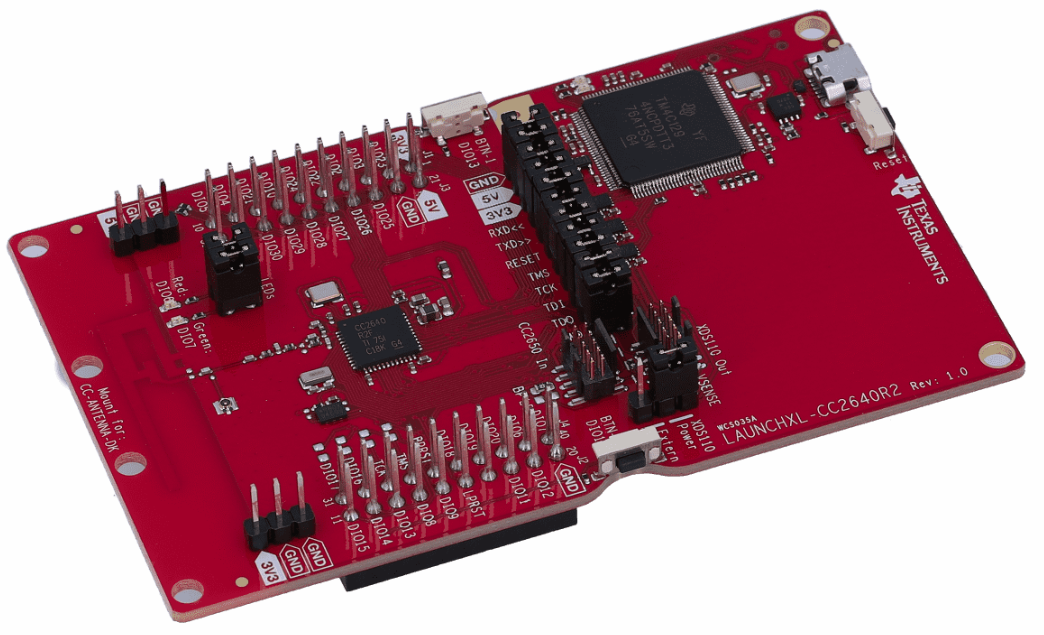
\includegraphics[width=.6\textwidth]{./Figures/LaunchpadCC2640R2.png}
	\caption{Kit de desarrollo launchpad CC2640R2.}
	\label{fig:kitDesarrolloCC2640R2}
\end{figure}

%\vspace{1cm}
